\section{Advanced MPI and boundary exchange optimisations}


\chapterDescription
  {
    The techniques discussed here are rather technical and/or non-trivial to
    implement, so realising them can be time-consuming.
  }
  {
    A working MPI code that scales to some degree.
  }



\subsection{Temporarily switch off vertex data exchange}
\label{section:64_advanced-mpi:switch-off-vertex-data-exchange}

\begin{smell}
  The performance analysis identifies that some ranks slow down the computation
  as they send out their boundary data late, i.e.~others have to wait. When we
  study the distribution of the runtime of the involved ranks, we see that a
  significand rato of the per-traversal runtime is spent on boundary data
  exchange.
\end{smell}


\begin{center}
  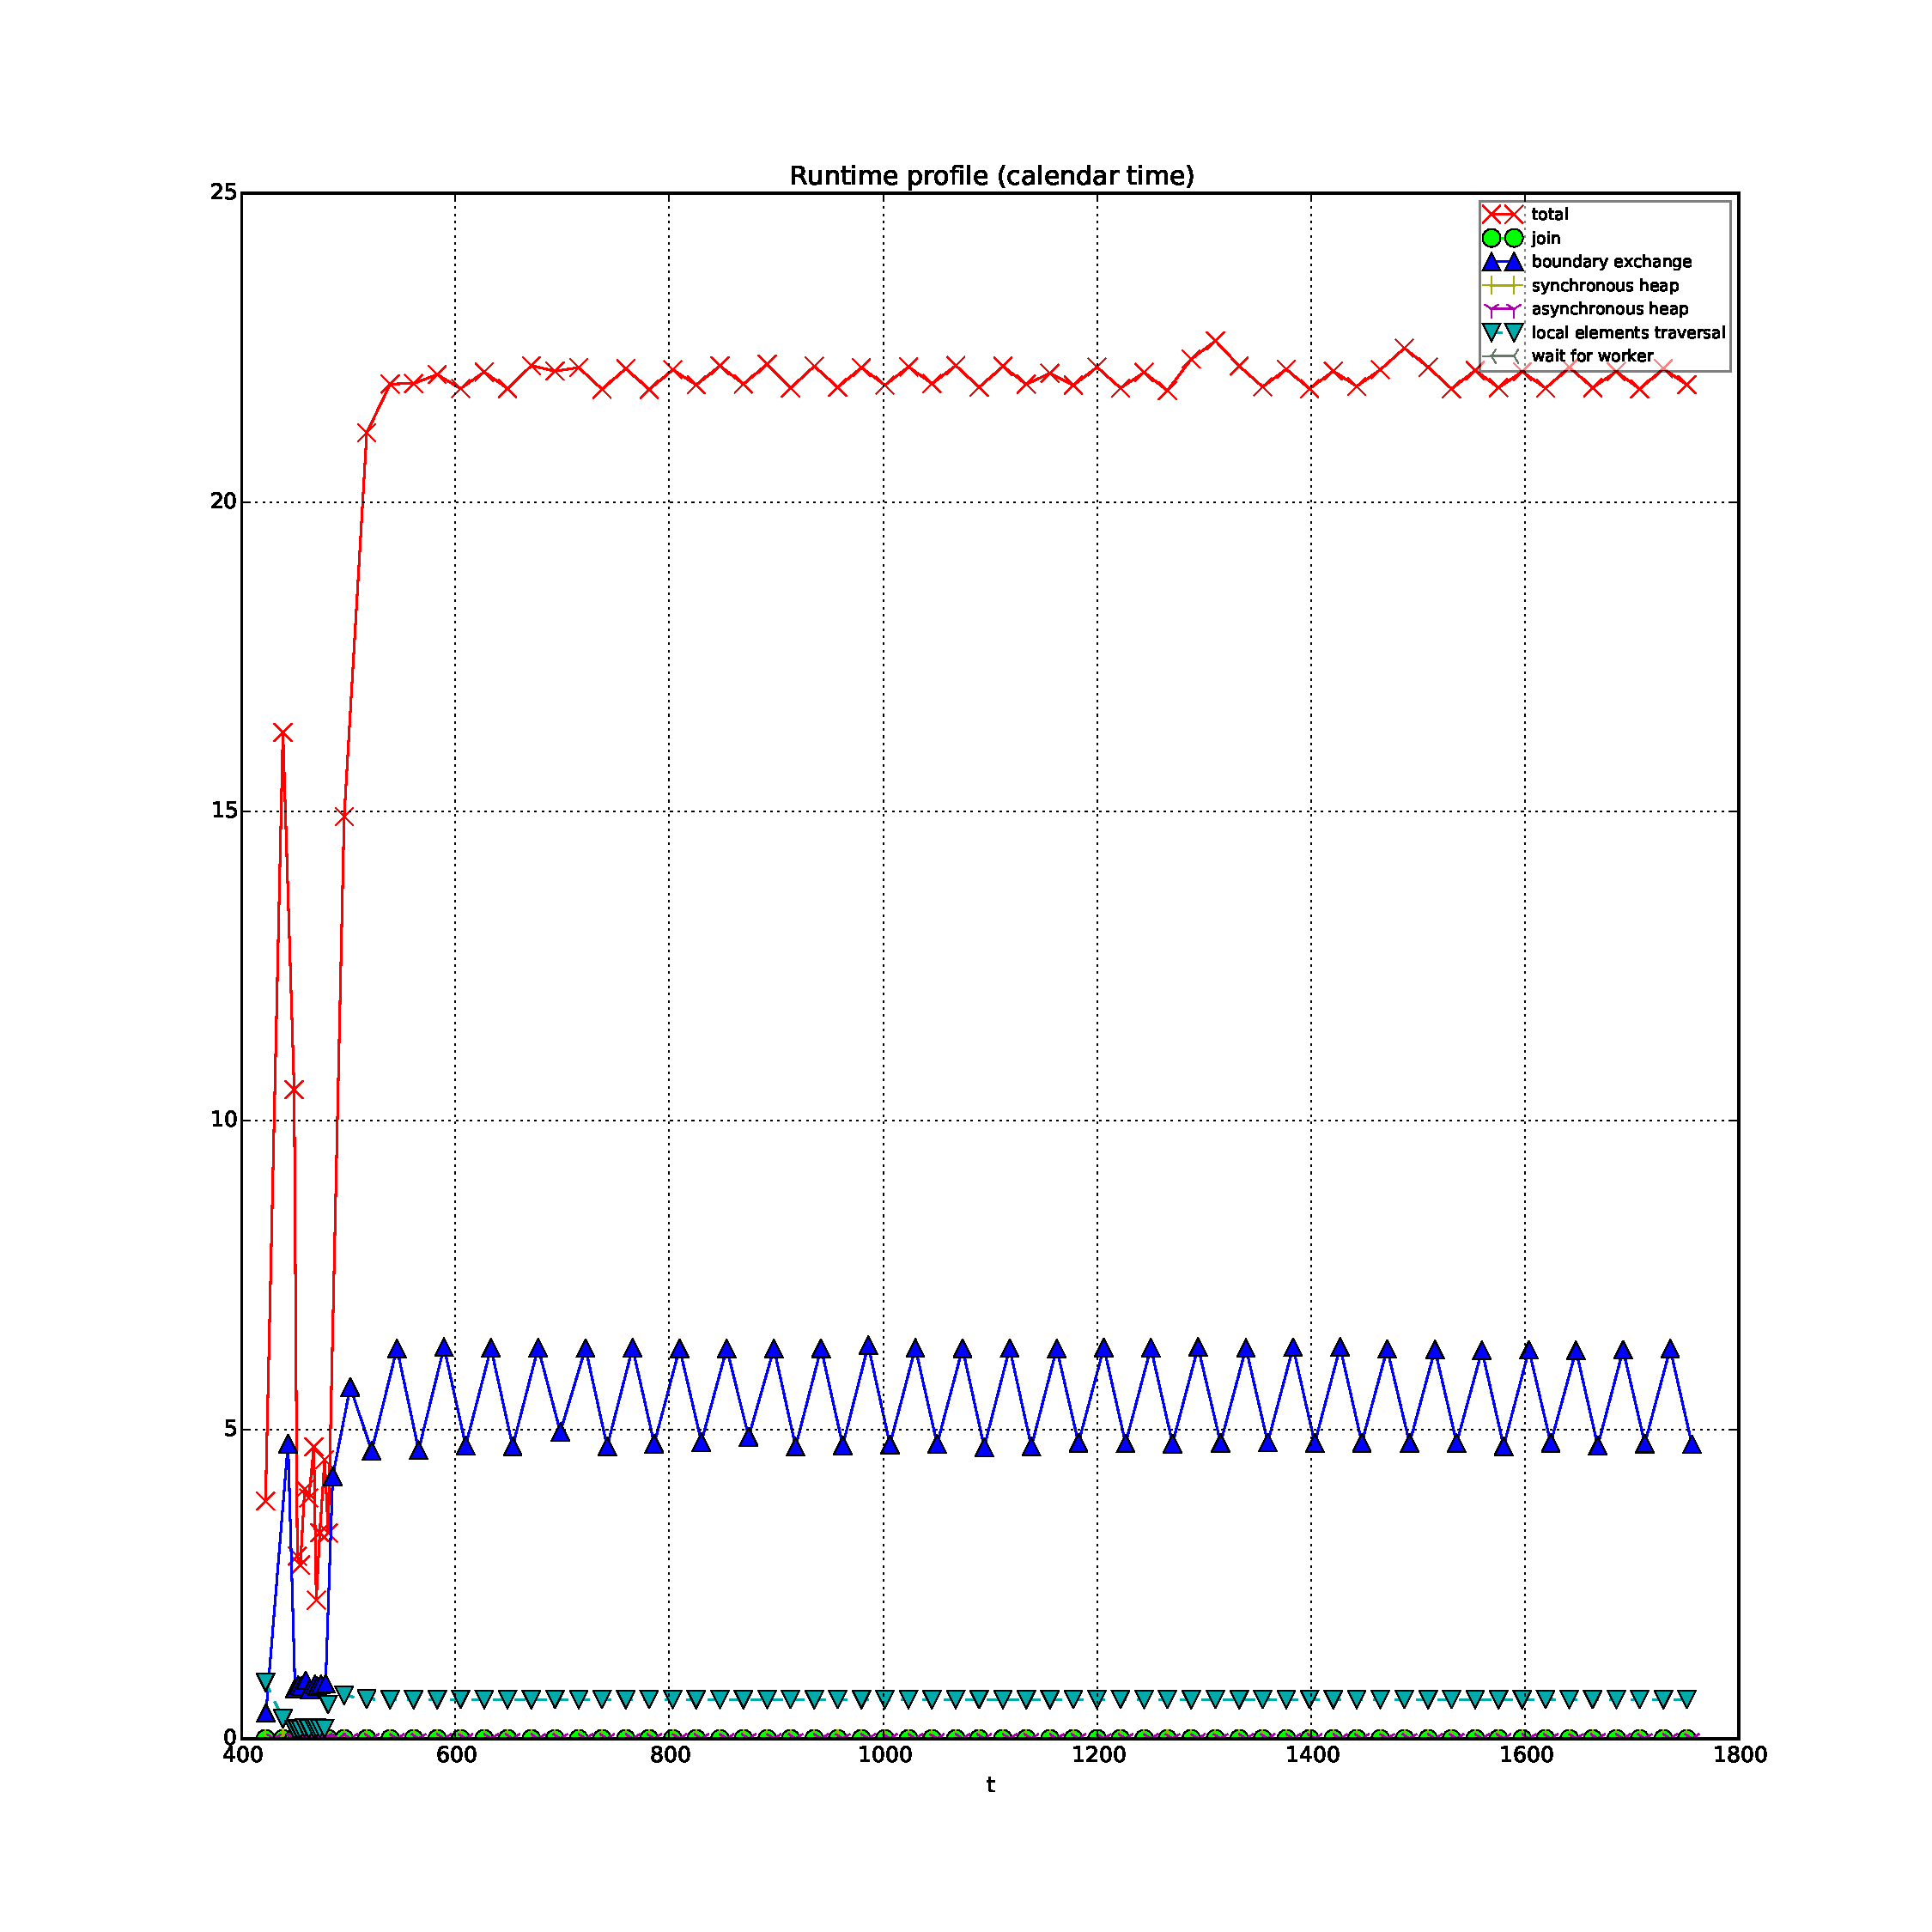
\includegraphics[width=0.5\textwidth]{64_advanced-mpi/boundary-exchange.pdf}
\end{center}


\noindent
We observe such a behaviour typically if the computational load per rank is low
(as we use low order finite elements, e.g.) or if all massive data exchange is
realised through heaps.
Heaps allow Peano to realise a more efficient data exchange than the standard
stack-based grid data, but they cannot communicate grid changes.

If we see such a pattern, it is worth to evaluate whether you can (temporarily)
switch off the data exchange and make the ranks work autonomously.
Peano passes control information along the MPI topology from masters to workers. 
We can switch off boundary data exchange on the first rank, i.e.~the global
master, and then this information is automatically propagated down to all the
ranks: all switch off the boundary exchange.

Peano realises a Jacobi-style boundary data exchange. 
Boundary data of one iteration is sent out throughout or, the latest, at the end
of the traversal.
Prior to the next traversal, this data is received. 
If we trigger a refine along a parallel boundary, this refine will thus become
active only in the subsequent iteration, when all ranks that hold a replicate of
the vertex have received copies of this vertex from all other ranks.
If we thus switch off the boundary data exchange, the next traversal still
receives vertices as they have been sent out the traversal before.
It however does not send out any data anymore.
In the second traversal (if we haven't switched on the boundary exchange again),
not data is exchanged anymore at all.
If we switch on the boundary data exchange again, the subsequent traversal sends
out grid data along the domain boundaries. 
Only in the second iteration after the switch on, both data is received and sent
out again.

While the description above claims that the boundary exchange control state is
exchanged via the state, we have to clarify that it is the repositories' state,
not the application-specific state. This is the state that also carries
information which adapter to run, e.g.
Therefore, the switch off is realised via the repository's \texttt{iterate}
command. 

\begin{code}
// on global master
const bool switchOffBoundaryExchange = true;
const int  numberOfIterationsToRunInOneRush = 10;
myRepository.iterate(numberOfIterationsToRunInOneRush,switchOffBoundaryExchange);
\end{code}

\noindent
The snippet runs one iteration where only boundary data is received but no
iteration is sent out anymore.
It then runs nine iterations where neither data is sent out nor received along
the boundary (from the grid; any heap data exchange is not affected).

Please note that the boundary data exchange is not switched off before you call 
\begin{code}
myRepository.iterate(...,false);
\end{code}
\noindent
once more. As soon as a \texttt{false} is passed, the subsequent first iteration
will not receive anything but send out boundary data. 
The iteration after, all communication, i.e.~both in and out, then is again
happening.



\begin{remark}
  If you switch off boundary data exchange, no load balancing can take place.
  Please also ensure that you switch off the exchange if and only if no
  rebalancing is going on, i.e.~the iteration before no rank has been joining or
  forking. 
  Otherwise, Peano will crash (with an assertion if compiled with asserts).
\end{remark}


\noindent
Peano does exchange vertices along the boundary after each grid sweep. 
It then compares all the refinement flags and performs the actual refinement.
This way, the grid remains consistent over all ranks: first, all refinement
information is exchanged. 
Once all ranks have received this information, the actual refinement is done.

If we switch off boundary exchange, obviously no refinement should ever be done
along domain boundaries as refinement triggers are not kept consistent.
Peano does switch off the refinement automatically, but you have to be aware how
a switch off of boundary information might affect your adaptivity patterns.

If a code triggers a refinement along a parallel domain boundary while
communication is switched off, this refinement does not pass through.
However, the refinement flag still is set. 
This means:
\begin{itemize}
  \item As soon as you reactive boundary data exchange, the code actually
  exchanges the refinement request. In the subsequent iteration, it then
  refines.
  \item The state remains instationary, i.e.~the state's \texttt{isGridBalanced}
  and \texttt{isGridStationary} return \texttt{false} as soon as the refinement
  is requested though it does not pass through.
\end{itemize}



\subsection{Deploying cores to MPI data exchange}
If you have parallelised your code with shared memory besides MPI, you can use
multithreaded MPI data exchange. 
This feature is switched off by the autogenerated makefile by default since
still some MPI implementations struggle to support multithreaded MPI commands.
It does so by defining the compile symbol
\texttt{-DnoMultipleThreadsMayTriggerMPICalls}.
Change this flag into \texttt{-DMultipleThreadsMayTriggerMPICalls} and
recompile.

Peano uses the threads in the background.
There is no change of any of your software required typically.
However, the impact on the runtime has to be evaluated carefully.





\subsection{Tailor the heap's data exchange}

This subsection's discussion applies only if you use the heap to exchange data.

\begin{smell}
  The code works reasonably well for small problem sizes, but starts to stall or
  perform really bad if the problem size increases.
\end{smell}


\noindent
Often, Peano users report that their code works fine for 2d problems. Once they
switch to 3d, they however experience massive scaling problems.

One of the issues with the heaps is that heaps split up all data exchange into
two types of messages. 
Some tiny meta data is exchanged first. 
It encodes per send how many real data entries are exchanged.
If your code triggers lots of sends with zero data (as data is held only on one
level or not by all vertices, e.g.), this means that lots of meta data is
roaming through your system while the actual big data messages are still fine.

How the meta data are handled depends on the type of boundary data exchange you
select in your heap.
Peano's plain heaps are straightforward and basically send out one integer message per 
send call before the actual data exchange is triggered.
If lots of sends do not actually transfer data (get passed 0), this means lots of zeros 
dripple through the network.

Peano also offers RLE variants of the heaps (runtime lenght encoding).
Those guys do not send out zero-lenght messages.
Instead they track all the messages of lenght zero that are sent one after
another.
Once real data is sent out, they first inform their communication partners that 
a number of empty messages without data has been hold back, before the actual
data goes out.
This obviously reduces the network usage.



\subsection{Avoid heap memory footprint explosions}

This subsection's discussion applies only if you use the heap to exchange data.

\begin{smell}
  The code works reasonably well for small problem sizes, but starts to consume 
  an unreasonable amount of memory once I scale up.
\end{smell}

\noindent
By default, Peano's heap does copy all data into a local buffer if you call \texttt{send}.
The framework realises some kind of buffered MPI.
While this is nice from a programmer's point of view---you don't have to care about
data consistency and almost all operations can be done in the background---it means
that the memory footprint can grow dramatically if lots of data is exchanged.


If you know that your data does not change its position in memory after you've 
called send---this is for example typically the situation when you send out data in 
\texttt{touchVertexLastTime}---you can instantiate the heap with zero copying.
Heaps are templates
\begin{code}
template<class Data, bool CreateCopiesOfSentData>
class PlainBoundaryDataExchanger;
\end{code} 
relying on boundary exchangers. The boundary exchanger types are responsible 
for the copying. 
So if you hand in \texttt{false} in the example above, you should get away
with a smaller memory footprint.




\subsection{Tailor data exchange format}
\label{section:advanced-mpi:tailor-data-exchange-format}

\begin{smell}
 The code's performance is low though the network bandwidth is definitely not
 the limiting factor.
\end{smell}


Peano internally offers two data formats for each individual piece of data
modelled through the \texttt{.def} files:
One variant works with plain C++ data types. 
This is the variant all Peano code parts (mappings, e.g.) are exposed to.
The other variant is a {\em packed} storage format where Peano squeezes out
all padding bytes (used to get the alignment right), merges multiple booleans
into one bit field, eliminates all temporary data, and so forth.
The latter format is used to store data in-between two grid iterations.
It also is, by default, used as MPI data exchange format.
If bandwidth is not an issue, you might profit from using plain C++ data types
for all data exchange which eliminates all overhead to convert the records forth
and back.
This is controlled via the compiler arguments

\begin{itemize}
  \item \texttt{-DnoParallelExchangePackedRecordsAtBoundary}
  \item \texttt{-DnoParallelExchangePackedRecordsBetweenMasterAndWorker}
  \item \texttt{-DnoParallelExchangePackedRecordsInHeaps}
  \item \texttt{-DnoParallelExchangePackedRecordsThroughoutJoinsAndForks}
\end{itemize}


\noindent
If you use \texttt{-DnoPackedRecords} this has obviously the same effect as
using the four flags but furthermore disables any efficient storage in the code.
Usually, doing so is not a good idea as it increases the memory footprint.


\begin{remark}
Some MPI versions struggle to cope with packed MPI records.
See entry in the troubleshooting section.
They then can be made working without packed records through these flags.
\end{remark}


